\documentclass[aspectratio=43,11pt]{beamer}
\usetheme{default}
\usecolortheme{default}
\setbeamertemplate{navigation symbols}{}
\setbeamertemplate{footline}[frame number]
\setbeamertemplate{itemize items}[circle]
\usepackage{xcolor}
\definecolor{maroon}{HTML}{500000}
\setbeamercolor{structure}{fg=maroon}

\usepackage[T1]{fontenc}
\usepackage{lmodern}
\usepackage{soul}
\usepackage{booktabs}
\usepackage{array}
\usepackage{listings}
\usepackage{tikz}
\usetikzlibrary{positioning,arrows.meta}
\lstset{basicstyle=\ttfamily\scriptsize, columns=fullflexible, keepspaces=true,
        showstringspaces=false, breaklines=true}


\title{Mini-Project: Instructions}
\subtitle{data prep $\rightarrow$ ML $\rightarrow$ optimization}
\author{DAEN 300 - Fall 2026}
\date{}
\titlegraphic{\IfFileExists{TAMU_logo.png}{
\includegraphics[height=1.2cm]{TAMU_logo.png}}{}}

\begin{document}

\begin{frame}
  \titlepage
\end{frame}

%===============================================================
\begin{frame}{Goal and timeline}
  \textbf{Goal:} use FEMA data to understand, step by step:
  \begin{enumerate}
    \item Who is more likely to get a home \textbf{inspection}? (\texttt{inspnReturned})
    \item Who is \textbf{eligible for repair assistance}? (\texttt{repairAssistanceEligible})
    \item How much \textbf{damage} FEMA found (\texttt{rpfvl}) vs.\ how much
          \textbf{repair money} people received (\texttt{repairAmount})
  \end{enumerate}
  \vspace{0.3em}
  Look for differences by \textbf{type of house}, \textbf{insurance},
  \textbf{how people registered}, \textbf{flooding}, and \textbf{disaster}.
  \vspace{0.6em}
  \begin{center}
  \begin{tabular}{@{}lll@{}}
    \toprule
    Day & Focus & Deliverable \\
    \midrule
    1 & Get data, explore, plan & Data dictionary + plan \\
    2 & Build models, measure, conclude & Notebook + conclusions \\
    \bottomrule
  \end{tabular}
  \end{center}
\end{frame}

%---------------------------------------------------------------
\begin{frame}{Getting the data}
  OpenFEMA: IHP Valid Registrations v2 \\
  {\tiny\url{https://www.fema.gov/openfema-data-page/individuals-and-households-program-valid-registrations-v2}}

  \vspace{0.8em}
  \textbf{Pick 2--4 large disasters} (many registrations), for example major
  hurricanes or floods. Write down their \texttt{disasterNumber}.

  \vspace{0.8em}
  Two ways to get them, choose one:
  \begin{itemize}
    \item \textbf{Option A: Download the CSV} from the data page
          (several GB!), then keep only your disasters while reading it
    \item \textbf{Option B: Use the API} to ask FEMA for only your
          disasters and columns
  \end{itemize}

  \vspace{0.8em}
  \small\emph{Honest note: I have not used this API much myself.
  Explore it, try things, and share what works!}
\end{frame}

%---------------------------------------------------------------
\begin{frame}[fragile]{Option A, download the CSV}
  The full file is too big to open at once. Read it \textbf{in pieces}
  and keep only the rows and columns you need:
\begin{lstlisting}
import pandas as pd

cols = ["disasterNumber", "residenceType", "ownRent",
        "homeOwnersInsurance", "floodInsurance", "registrationMethod",
        "grossIncome", "householdComposition", "applicantAge",
        "primaryResidence", "selfAssessmentInformation",
        "inspnIssued", "inspnReturned", "rpfvl", "waterLevel",
        "highWaterLocation", "floodDamage", "foundationDamage",
        "roofDamage", "destroyed", "habitabilityRepairsRequired",
        "repairAssistanceEligible", "repairAmount"]
my_disasters = [4332, 4673]                # your choice

parts = []
for chunk in pd.read_csv("IHP.csv",        # your file name
                         usecols=cols, chunksize=500_000):
    parts.append(chunk[chunk["disasterNumber"].isin(my_disasters)])

df = pd.concat(parts, ignore_index=True)
df.to_parquet("ihp.parquet")                 # fast to reload later
\end{lstlisting}
\end{frame}

%---------------------------------------------------------------
\begin{frame}[fragile]{Option B, use the API}
  The API returns at most 10,000 rows per request, so ask for
  ``pages'' until nothing comes back:
\begin{lstlisting}
import requests, pandas as pd

url = ("https://www.fema.gov/api/open/v2/"
       "IndividualsAndHouseholdsProgramValidRegistrations")
params = {
    "$select": ",".join(cols),          # cols from Option A
    "$filter": "disasterNumber eq 4332 or disasterNumber eq 4673",
    "$orderby": "id",
    "$top": 10000,
    "$skip": 0,
}
pages = []
while True:
    data = requests.get(url, params=params, timeout=120).json()
    rows = data["IndividualsAndHouseholdsProgramValidRegistrations"]
    if not rows: break                  # no more pages
    pages.append(pd.DataFrame(rows))
    params["$skip"] += 10000

df = pd.concat(pages, ignore_index=True)
df.to_parquet("ihp.parquet")
\end{lstlisting}
\end{frame}

%---------------------------------------------------------------
\begin{frame}[fragile]{Import and first look}
\begin{lstlisting}
df = pd.read_parquet("ihp.parquet")

df.shape                                   # rows, columns
df.info()                                  # types and missing values
df.describe()                              # numeric summaries
df["disasterNumber"].value_counts()        # rows per disaster
df["residenceType"].value_counts()         # types of houses
df.groupby("disasterNumber")["inspnReturned"].mean()   # inspection rate
\end{lstlisting}
  \vspace{0.5em}
  \begin{itemize}
    \item Do the numbers make sense? Any strange codes or missing values?
    \item Compare disasters early: they can be very different
  \end{itemize}
\end{frame}

%===============================================================
\section{Day 1}

\begin{frame}
  \centering
  \Huge Day 1 \\[0.5em]
  \large Get data $\cdot$ Explore $\cdot$ Plan
\end{frame}

\begin{frame}{Day 1 goals}
  By the end of class you should:
  \vspace{0.5em}
  \begin{enumerate}
    \item Download and import your disasters; record a \textbf{baseline}
          (time, rows, memory)
    \item Know every variable you will use: \textbf{type, meaning, missing values}
    \item Explore \textbf{inspection} first, then \textbf{eligibility} and
          \textbf{amounts}, with tables and plots
    \item Decide which variables to use for each question
    \item Submit a \textbf{plan}: architecture diagram \emph{and} pseudocode
  \end{enumerate}
\end{frame}

%---------------------------------------------------------------
\begin{frame}{1.1 Load and measure a baseline}
  \begin{itemize}
    \item Load your data \textbf{as-is} (default types)
    \item Record:
      \begin{itemize}
        \item download / load time (\texttt{\%time} or \texttt{\%timeit})
        \item number of rows and columns
        \item memory: \texttt{df.memory\_usage(deep=True).sum()}
      \end{itemize}
    \item Keep these numbers --- they are your ``before'' on Day 2
  \end{itemize}
  \vspace{0.8em}
  \begin{center}
  \begin{tabular}{@{}lll@{}}
    \toprule
    Measure & Baseline & After (Day 2) \\
    \midrule
    Load time (s) & & \\
    Rows $\times$ columns & & \\
    Memory (MB) & & \\
    \bottomrule
  \end{tabular}
  \end{center}
\end{frame}

%---------------------------------------------------------------
\begin{frame}{1.2 Variables to study}
  \footnotesize
  \begin{tabular}{@{}>{\raggedright\arraybackslash}p{0.27\textwidth}>{\raggedright\arraybackslash}p{0.68\textwidth}@{}}
    \toprule
    Group & Variables \\
    \midrule
    \textbf{Household} \newline (known at registration)
      & \texttt{residenceType}, \texttt{ownRent}, \texttt{homeOwnersInsurance},
        \texttt{floodInsurance}, \texttt{registrationMethod}, \texttt{grossIncome},
        \texttt{householdComposition}, \texttt{applicantAge}, \texttt{primaryResidence} \\[0.3em]
    \textbf{Self-reported} damage
      & \texttt{selfAssessmentInformation} \\[0.3em]
    \textbf{Inspection} results \newline (known after inspection)
      & \texttt{rpfvl}, \texttt{waterLevel}, \texttt{highWaterLocation},
        \texttt{floodDamage}, \texttt{foundationDamage}, \texttt{roofDamage},
        \texttt{destroyed}, \texttt{habitabilityRepairsRequired} \\[0.3em]
    \textbf{Outcomes}
      & \texttt{inspnReturned}, \texttt{repairAssistanceEligible}, \texttt{repairAmount} \\[0.3em]
    \textbf{Disaster}
      & \texttt{disasterNumber} \\
    \bottomrule
  \end{tabular}
  \vspace{0.8em}
  \normalsize
  \begin{itemize}
    \item \texttt{rpfvl} = damage FEMA \textbf{assessed};
          \texttt{repairAmount} = money \textbf{received}
    \item Found another useful variable? Add it and explain why
  \end{itemize}
\end{frame}

%---------------------------------------------------------------
\begin{frame}{1.3 Build a data dictionary}
  Fill one row per variable you keep:
  \vspace{0.5em}
  \begin{center}
  \scriptsize
  \begin{tabular}{@{}lllll@{}}
    \toprule
    Field & Type & Meaning & \% miss. & Known when? \\
    \midrule
    \texttt{ownRent} & object & O / R / unknown & & registration \\
    \texttt{residenceType} & & & & \\
    \texttt{homeOwnersInsurance} & & & & \\
    \texttt{registrationMethod} & & & & \\
    \texttt{waterLevel} & & & & after inspection \\
    \texttt{rpfvl} & & & & after inspection \\
    \dots & & & & \\
    \bottomrule
  \end{tabular}
  \end{center}
  \vspace{0.5em}
  \begin{itemize}
    \item Use the OpenFEMA data page for definitions
    \item ``Known when?'' decides which question each variable can help answer
  \end{itemize}
\end{frame}

%---------------------------------------------------------------
\begin{frame}{1.4 Explore inspection first}
  \textbf{Question:} who has a better chance of being inspected?
  \vspace{0.5em}
  \begin{enumerate}
    \item What share of registrations were inspected? In each disaster?
    \item Inspection rate by \texttt{residenceType} and \texttt{ownRent}
    \item With vs.\ without \texttt{homeOwnersInsurance} or \texttt{floodInsurance}
    \item By \texttt{registrationMethod} (phone, internet, mobile, \dots)
    \item By \texttt{grossIncome} and \texttt{selfAssessmentInformation}
  \end{enumerate}
  \vspace{0.5em}
  \textbf{Tools:} \texttt{groupby(...).mean()}, \texttt{pd.crosstab},
  bar charts. \\
  Show each result \textbf{per disaster}: does the pattern hold in all of them?
\end{frame}

%---------------------------------------------------------------
\begin{frame}{1.5 Then explore eligibility and amounts}
  Use only \textbf{inspected} homes:
  \vspace{0.5em}
  \begin{enumerate}
    \item Eligibility rate by \texttt{residenceType}, insurance,
          \texttt{floodDamage}, \texttt{destroyed}
    \item \texttt{rpfvl} vs.\ \texttt{waterLevel}: scatter plot.
          Does more water mean more damage?
    \item \texttt{rpfvl} (assessed) vs.\ \texttt{repairAmount} (received):
          how close are they?
    \item How many zeros? Histograms of the amounts and of
          \texttt{np.log1p(amount)}
    \item Correlation heatmap of the numbers and yes/no variables
          (\texttt{df.corr()})
  \end{enumerate}
  \vspace{0.5em}
  Again, compare \textbf{across disasters}.
\end{frame}

%---------------------------------------------------------------
\begin{frame}{1.6 Which variables for which question?}
  \textbf{Rule:} use only what is known \emph{before} the outcome.
  \vspace{0.6em}
  \begin{center}
  \footnotesize
  \begin{tabular}{@{}lll@{}}
    \toprule
    Question & Rows & Variables \\
    \midrule
    1. Inspected? & all registrations & household + disaster \\
    2. Eligible? & inspected only & household + inspection + disaster \\
    3. Amount received? & eligible only & household + inspection + disaster \\
    \bottomrule
  \end{tabular}
  \end{center}
  \vspace{0.6em}
  \begin{itemize}
    \item Do \textbf{not} use \texttt{rpfvl} or \texttt{waterLevel} to explain inspection
          --- they come from the inspection itself
    \item Do \textbf{not} use other award amounts as inputs
    \item \textbf{Control by disaster}: include \texttt{disasterNumber}
          as a variable, and check results per disaster
    \item Write one sentence explaining each variable you keep
  \end{itemize}
\end{frame}

%---------------------------------------------------------------
\begin{frame}{1.7 Plan: architecture diagram (example)}
  \centering
  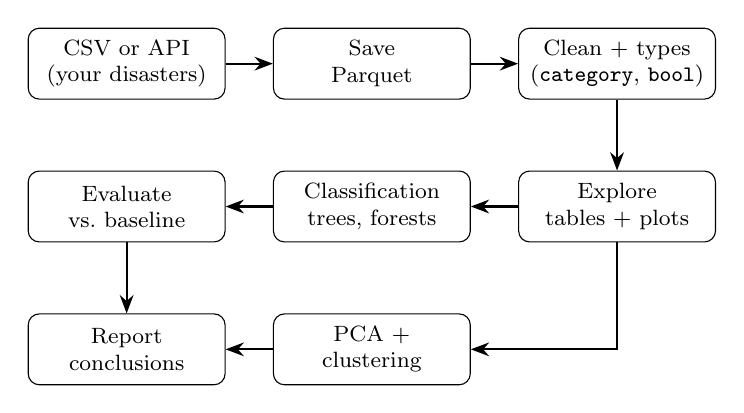
\begin{tikzpicture}[
      box/.style={draw, rounded corners, align=center, minimum width=2.5cm,
                  minimum height=0.9cm, font=\footnotesize},
      arr/.style={-{Stealth}, thick}]
    \node[box] (api) {CSV or API\\(your disasters)};
    \node[box, right=0.6cm of api] (raw) {Save\\Parquet};
    \node[box, right=0.6cm of raw] (clean) {Clean + types\\(\texttt{category}, \texttt{bool})};
    \node[box, below=0.9cm of clean] (eda) {Explore\\tables + plots};
    \node[box, left=0.6cm of eda] (ml) {Classification\\trees, forests};
    \node[box, left=0.6cm of ml] (eval) {Evaluate\\vs.\ baseline};
    \node[box, below=0.9cm of ml] (pca) {PCA +\\clustering};
    \node[box, below=0.9cm of eval] (rep) {Report\\conclusions};
    \draw[arr] (api) -- (raw);
    \draw[arr] (raw) -- (clean);
    \draw[arr] (clean) -- (eda);
    \draw[arr] (eda) -- (ml);
    \draw[arr] (ml) -- (eval);
    \draw[arr] (eda) |- (pca);
    \draw[arr] (eval) -- (rep);
    \draw[arr] (pca) -- (rep);
  \end{tikzpicture}\par
  \vspace{0.8em}
  \raggedright
  \small Draw \emph{your own}: mark where you will \textbf{measure} time or memory.
\end{frame}

%---------------------------------------------------------------
\begin{frame}[fragile]{1.8 Plan: pseudocode (template/example)}
\begin{lstlisting}
GET data for my disasters (CSV in chunks, or API pages)
SAVE as parquet;  RECORD time, rows, memory

PREPARE:
    set types (category, bool);  handle missing values
    one-hot encode categories (incl. disasterNumber)

Q1 inspected?    rows = all        X = household + disaster
Q2 eligible?     rows = inspected  X = household + inspection + disaster
Q3 repairAmount? rows = eligible   X = same as Q2

FOR each question:
    split train / test
    fit BASELINE                 -> record score
    fit linear model             -> record score
    (if time) fit logistic       -> record score
    fit tree, random forest      -> record score, top features
    CHECK results per disaster

PCA (2 components) + k-means on inspected homes
DESCRIBE each cluster
REPORT before/after table, plots, conclusions
\end{lstlisting}
\end{frame}

%---------------------------------------------------------------
\begin{frame}{Day 1 deliverable (Fri Nov 13)}
  Submit on Canvas (notebook (and its PDF export) or just PDF):
  \vspace{0.5em}
  \begin{itemize}
    \item[$\square$] Which disasters you chose, and why
    \item[$\square$] Baseline table: time, rows, memory
    \item[$\square$] Data dictionary for every variable you keep
    \item[$\square$] Exploration of inspection, then eligibility and amounts
          (tables/plots with one-line takeaways)
    \item[$\square$] Variables chosen for each question
    \item[$\square$] Architecture diagram (hand-drawn photo is fine, or draw.io)
    \item[$\square$] Pseudocode or algorithm for the full workflow
    \item[$\square$] One or two things you want to try to make faster or lighter
  \end{itemize}
\end{frame}

%===============================================================
\section{Day 2}

\begin{frame}
  \centering
  \Huge Day 2 \\[0.5em]
  \large Build models $\cdot$ Measure $\cdot$ Conclude
\end{frame}

\begin{frame}{Day 2 goals}
  By the end of class you should:
  \vspace{0.5em}
  \begin{enumerate}
    \item Implement your Day 1 plan (update it if it changed)
    \item Try a few speed/memory improvements and \textbf{measure} them
    \item Build and evaluate models for the three questions, against a
          \textbf{baseline}
    \item Use PCA and clustering to find \textbf{groups} of similar households
    \item Write \textbf{conclusions} supported by your numbers
  \end{enumerate}
\end{frame}

%---------------------------------------------------------------
\begin{frame}{2.1 Optimization: learn by doing}
  \textbf{Try it, measure it, keep what helps.} No need for big changes.
  \vspace{0.5em}
  \begin{itemize}
    \item Read fewer columns; change types to \texttt{category} and \texttt{bool}
          --- how much memory did you save?
    \item Reload from Parquet instead of CSV --- how much faster?
    \item Find one slow step with \texttt{\%prun}; replace a loop or
          \texttt{.apply()} with a vectorized version or \texttt{groupby}
    \item Random forest slow? Try \texttt{n\_jobs=-1} or fewer trees
  \end{itemize}
  \vspace{0.5em}
  \begin{center}
  \footnotesize
  \begin{tabular}{@{}llll@{}}
    \toprule
    What I tried & Before & After & Worth it? \\
    \midrule
    \texttt{category} types & \dots MB & \dots MB & \\
    Parquet reload & \dots s & \dots s & \\
    \dots & & & \\
    \bottomrule
  \end{tabular}
  \end{center}
\end{frame}

%---------------------------------------------------------------
\begin{frame}{2.2 Simple classification and evaluation}
  Questions 1 and 2 (inspected? eligible?):
  \vspace{0.4em}
  \begin{itemize}
    \item \textbf{Baseline}: always predict the most common answer
    \item \textbf{Simple model}: linear regression on the 0/1 outcome
          (any linear approach from class is fine); predict ``yes''
          if the result is $\ge 0.5$
    \item \textbf{If time allows}: try logistic regression and compare
    \item \textbf{Evaluate} on a test set:
      \begin{itemize}
        \item confusion matrix
        \item accuracy, precision, recall, F1
        \item cross-validation (\texttt{cross\_val\_score})
      \end{itemize}
    \item Are the classes balanced? If not, accuracy can fool you
  \end{itemize}
  \vspace{0.4em}
  Question 3 (amount): linear regression on \texttt{repairAmount}\\
  {\footnotesize ex: \texttt{np.log1p(repairAmount)}; report MAE, RMSE, predicting the mean.}
\end{frame}

%---------------------------------------------------------------
\begin{frame}{2.3 Decision trees and random forests}
  \begin{itemize}
    \item \textbf{Decision tree}: try depths 2, 4, 8, \dots
      \begin{itemize}
        \item plot train vs.\ test score by depth --- where does it start to overfit?
        \item draw a small tree (depth 2--3): can you explain its rules in words?
      \end{itemize}
    \item \textbf{Random forest}: compare with the single tree
    \item \textbf{Feature importance}: which variables matter most?
      \begin{itemize}
        \item house type? insurance? registration method? water level?
      \end{itemize}
    \item Use \texttt{DecisionTreeRegressor} / \texttt{RandomForestRegressor}
          for \texttt{repairAmount}
    \item Same \textbf{evaluation} as 2.2, so you can compare all models in one table
  \end{itemize}
\end{frame}

%---------------------------------------------------------------
\begin{frame}{2.4 PCA and clustering}
  \textbf{Goal:} find groups of similar inspected households.
  \vspace{0.4em}
  \begin{enumerate}
    \item Scale the numeric variables (\texttt{StandardScaler})
    \item \textbf{PCA} to 2 components; plot them colored by eligibility
          and by disaster
    \item How much variance do 2 components explain?
    \item \textbf{k-means} with a few values of $k$; pick one and explain why
    \item Describe each cluster: house types, insurance, water level,
          \texttt{rpfvl}, eligibility rate, \texttt{repairAmount}
  \end{enumerate}
  \vspace{0.4em}
  \small Note: PCA reduces many variables to a few; k-means makes the groups.
\end{frame}

%---------------------------------------------------------------
\begin{frame}{2.5 Conclusions}
  Answer in short paragraphs, each backed by a number, table, or plot:
  \vspace{0.5em}
  \begin{enumerate}
    \item Who is more likely to be \textbf{inspected}, and to be
          \textbf{eligible}?
    \item How do outcomes differ by \textbf{type of house}, \textbf{insurance},
          \textbf{registration method}, and \textbf{flooding}?
    \item How does \texttt{repairAmount} (received) compare with
          \texttt{rpfvl} (assessed)?
    \item Do your findings hold \textbf{in every disaster}?
    \item How much better than the \textbf{baseline} is each model?
    \item Which optimization helped most?
    \item \textbf{Limitations} and what you would do with more time
  \end{enumerate}
\end{frame}

%---------------------------------------------------------------
\begin{frame}{Day 2 final deliverable (Fri Nov 20)}
  Submit on Canvas: one Jupyter notebook (and its PDF export)
  \vspace{0.5em}
  \begin{itemize}
    \item[$\square$] Updated plan (diagram + pseudocode), noting any changes
    \item[$\square$] Optimization table: what you tried, before/after
    \item[$\square$] Model comparison table (baseline, simple, tree, forest)
    \item[$\square$] Feature importance and PCA/cluster plots
    \item[$\square$] Conclusions
    \item[$\square$] Sources and AI use acknowledged
  \end{itemize}
  \vspace{0.8em}
  \hl{Presentation quality (organization, clarity, tables, graphs, discussion)
      is part of the grade.}
\end{frame}

\end{document}
